\documentclass[twoside]{article}

%\usepackage[math]{kurier}
\usepackage[sc]{mathpazo}                   
%\renewcommand{\sfdefault}{kurier}

\usepackage{mathtools}

\usepackage{graphics}
\setlength{\oddsidemargin}{0.25 in}
\setlength{\evensidemargin}{-0.25 in}
\setlength{\topmargin}{-0.6 in}
\setlength{\textwidth}{6.5 in}
\setlength{\textheight}{8.5 in}
\setlength{\headsep}{0.75 in}
\setlength{\parindent}{0 in}
\setlength{\parskip}{0.1 in}


\newcounter{lecnum}
\renewcommand{\thepage}{\thelecnum-\arabic{page}}
\renewcommand{\thesection}{\thelecnum.\arabic{section}}
\renewcommand{\theequation}{\thelecnum.\arabic{equation}}
\renewcommand{\thefigure}{\thelecnum.\arabic{figure}}
\renewcommand{\thetable}{\thelecnum.\arabic{table}}


\newcommand{\lecture}[4]{
   \pagestyle{myheadings}
   \thispagestyle{plain}
   \newpage
   \setcounter{lecnum}{#1}
   \setcounter{page}{1}
   \noindent
   \begin{center}
   \framebox{
      \vbox{\vspace{2mm}
    \hbox to 6.28in { {\bf  CS 294-115 Algorithmic Human-Robot Interaction
                        \hfill Fall 2016} }
       \vspace{4mm}
       \hbox to 6.28in { {{\Large \hfill Lecture #1: #2  \hfill}} }
       \vspace{2mm}
       \hbox to 6.28in { {\it \hfill Scribes: #4} }
      \vspace{2mm}}
   }
   \end{center}
   \markboth{Lecture #1: #2}{Lecture #1: #2}

   \vspace*{4mm}
}
% what is the third argument to this command for?

\newcommand{\ts}{\textsuperscript}
\newcommand{\cu}{\mathcal{U}}
\newcommand{\cus}{\mathcal{U}_\text{smooth}}

%%%%%%%%%%%%%%%%%%%%%%%%%%
%document
\begin{document}
\lecture{7}{Trajectory Optimisation Part III}{}{Daniel Filan and Davis Foote}

\section{Summary}
This lecture will have two sections: first, an explanation of why and how to change the inner product implicitly used to define functional gradient descent, and secondly, a discussion of how student paper presentations will work, and why they will work that way.

\section{Changing the inner product}
\label{sec:chang-inner-prod}

For ease of understanding, we will think about our trajectories as discretised vectors, whose $i$\ts{th} component is the position in configuration space of the trajectory at the $i$\ts{th} point in (discrete) time. This vector will look something like
\begin{equation}
  \label{eq:1}
  \xi =
  \begin{bmatrix}
    q_1 \\
    q_2 \\
    q_3 \\
    \vdots \\
    q_N
  \end{bmatrix}
\end{equation}
Since we won't consider changing the start or end points of the trajectory, we leave out the initial configuration $q_0$ and the final configuration $q_{N+1}$. We should also remember that each element of this vector is itself a vector, rather than simply a scalar.

So far, we have been using the Euclidean inner product, defined as
\begin{equation}
  \label{eq:2}
  \langle \xi_1, \xi_2 \rangle_E = \xi_1^{\top} \xi_2 = q_{1,1}^{\top}q_{2,1} + \dotsb + q_{1,N}^\top q_{2,N}
\end{equation}

Why would we want to change this? Well, an inner product defines a norm by $\|\xi\| = \sqrt{\langle \xi, \xi \rangle}$, and a norm defines a distance metric defined by $\text{distance}(\xi_1, \xi_2) = \| \xi_1 - \xi_2 \|$. Therefore, we might ask ourselves whether the Euclidean metric induced by the Euclidean inner product is any good.

\subsection{Why the Euclidean metric isn't good}
\label{sec:why-euclidean-metric}

Consider three trajectories of a robot with one degree of freedom:

\begin{center}
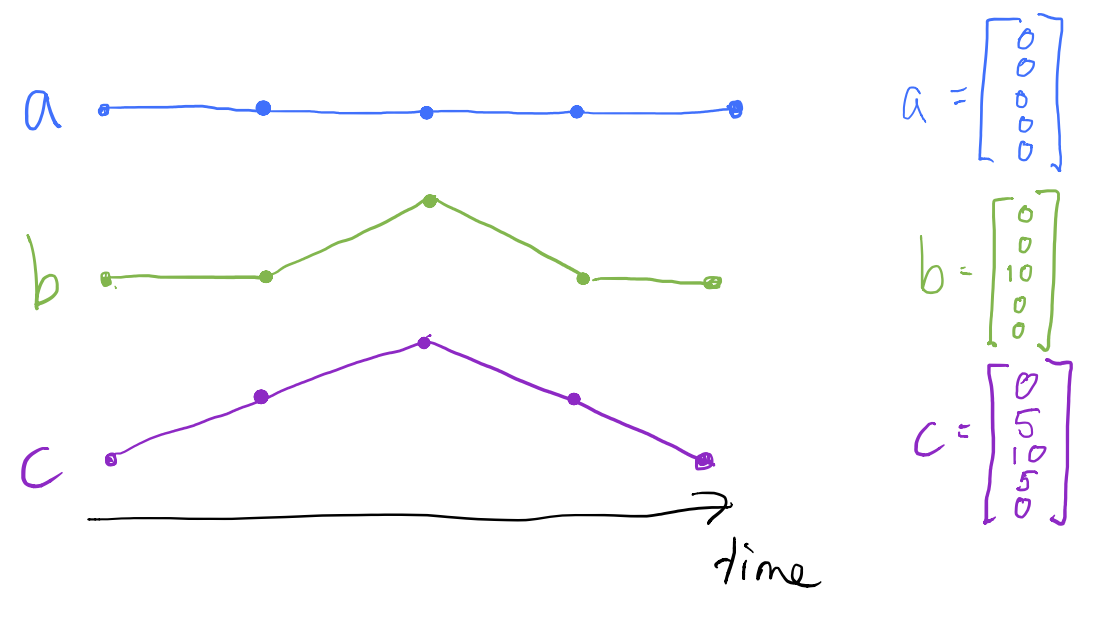
\includegraphics[scale=0.3]{figures/trajectory_illustration.png}
\end{center}

\begin{equation}
  \label{eq:3}
  a =
  \begin{bmatrix}
    0 \\
    0 \\
    0 \\
    0 \\
    0
  \end{bmatrix},\, b =
  \begin{bmatrix}
    0 \\
    0 \\
    10 \\
    0 \\
    0
  \end{bmatrix}, \text{ and } c =
  \begin{bmatrix}
    0 \\
    5 \\
    10 \\
    5 \\
    0
  \end{bmatrix}
\end{equation}

Which is closer to $a$: $b$ or $c$? Well,
\begin{equation}
  \label{eq:4}
  \|a - b \|^2_E = \langle b, b \rangle_E = 10 \times 10 = 100
\end{equation}
and
\begin{equation}
  \label{eq:5}
  \|a - c \|^2_E = \langle c, c \rangle_E = 5 \times 5 + 10 \times 10 + 5 \times 5 = 150
\end{equation}
Therefore, according to the Euclidean metric, $b$ is closer to $a$ than $c$ is. However, intuitively, there's something wrong with this. $a$ involves very smooth motion, $b$ is super jerky, and $c$ involves a bit of a jerk, but less so than $b$. The Euclidean metric can't notice this because it doesn't take the orderings of elements of the vector into account, and therefore can't talk about speeds, but it would be nice if we could take time into account somehow.

Can we give a more rigorous argument for why we should change metric?

\subsubsection{Detour 1}
\label{sec:detour-1-1}

The formula for gradient descent, as we know, is $\xi_{i+1} = \xi_i - (1/\alpha)\nabla_{\xi_i}\cu$. But where does this come from?

Suppose instead that we approximate $\cu$ by its first order Taylor expansion, and try to minimise that. Then, we would use the rule
\begin{align}
  \label{eq:6}
  \xi_{i+1} &= \text{arg min}_{\xi} \left\{ \cu[\xi_i] + \nabla_{\xi_i}\cu^{\top} (\xi - \xi_i)\right\}\\
  \intertext{However, we know that this Taylor expansion will be off if we get far away in norm from $\xi_i$, so we add a regularisation term to penalise this\footnotemark:}
  \xi_{i+1} &= \text{arg min}_{\xi} \left\{ \cu[\xi_i] + \nabla_{\xi_i}\cu^{\top} (\xi - \xi_i) + \frac{1}{2} \alpha \|\xi - \xi_i \|_E^2 \right\}\label{eq:7} \\
  \intertext{This is a quadratic problem in $\xi$, so we can take the gradient of the term inside the curly brackets, set the gradient to zero, and thereby solve the problem. Doing this, we get}
  &\phantom{= \text{arg min}_\xi \Bigg\{\,\, }0 + \nabla_{\xi_i}\cu + \alpha (\xi - \xi_i)\label{eq:9}
\end{align}
\footnotetext{Alternatively, we can arrive at this by considering a trust-region constraint where we set some bound on how far from $\xi_i$ we are allowed to move. If we write out the Lagrangian, we arrive at equation \eqref{eq:10} where $\alpha$ is the Lagrange multiplier.}
Setting that expression to 0, we obtain
\begin{equation}
  \label{eq:10}
  \xi_{i+1} = \xi_i - \frac{1}{\alpha} \nabla_{\xi_i} \cu
\end{equation}
which is exactly the formula for gradient descent.

\subsubsection{Back to the main track}
\label{sec:back-main-track}

Remember the example of vectors $a$, $b$, and $c$? Well, gradient descent tends to go to things that are closer in norm, all else being equal. So, if $b$ is closer to $a$ than $c$ is, even if $c$ is better than $b$, gradient descent might well reach $b$ first, because of how much further away $c$ is.

What's the solution? We will change the distance metric (by changing the inner product) so that the sphere of elements of constant distance away from $a$ becomes an ellipsoid, thereby making $c$ closer than $b$.

\begin{center}
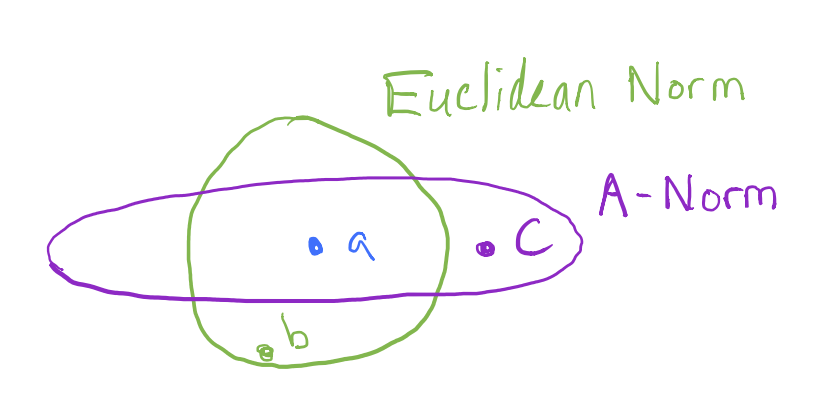
\includegraphics[scale=0.3]{figures/balls.png}
\end{center}

\subsection{How to make a new inner product}
\label{sec:how-make-new}

All inner products are of the form $\xi_1^\top A \xi_2$, where $A$ is a positive semi-definite matrix. Therefore, we just have to choose a matrix $A$. How?

Since we want our metric to like smooth deformations, let's think of other things that like that. Remember $\cus$? That was defined as
\begin{equation}
  \label{eq:11}
  \cus[\xi] = \frac{1}{2} \int_0^T \|\xi'(t)\|^2 dt
\end{equation}
When we discretise, the analogue of this is
\begin{equation}
  \cus[\xi] = \frac{1}{2} \sum_{i=0}^N \|q_{i+1} - q_i\|^2\label{eq:12}
\end{equation}

Suppose we compute the partial derivative of $\cus$ with respect to $q_i$. This is
\begin{equation}
  \label{eq:13}
  \frac{\partial}{\partial q_i}\cus = (\nabla_{\xi}\cus)_i = - (q_{i+1} - q_i) + (q_i - q_{i-1}) = 2q_i - q_{i-1} - q_{i+1}
\end{equation}
We're going to form a matrix $A$ such that
\begin{equation}
  \label{eq:14}
  \nabla_{\xi}\cus = A \xi + c
\end{equation}
where the constant $c$ will appear because $\nabla_\xi \cus$ depends on the endpoints $q_0$ and $q_{N+1}$, which don't appear in $\xi$. The matrix that does this is
\begin{equation}
  \label{eq:15}
  A =
  \begin{bmatrix}
    2 & -1 & & & & \\
    -1 & 2 & -1 & & & \\
    & -1 & 2 & -1 & & \\
    & & \ddots & \ddots & \ddots &  \\
    & & & -1 & 2 & -1 \\
    & & & & -1 & 2
  \end{bmatrix}
\end{equation}
This $A$ (the Hessian of $\cus$) will be what we use for our inner product:
\begin{equation}
  \label{eq:16}
  \langle \xi_1, \xi_2 \rangle_A = \xi_1^\top A \xi_2 \text{ and therefore } \|\xi_1 - \xi_2\|_A^2 = (\xi_1 - \xi_2)^\top A (\xi_1 - \xi_2)
\end{equation}

Going back to our motivational example, we now have that

\begin{align*}
  \|b - a\|^2_A &= \|b\|_A^2 \\
                &=
                  \begin{bmatrix}
                    0 & 0 & 10 & 0 & 0
                  \end{bmatrix}
                  \begin{bmatrix}
                    2 & -1 & 0 & 0 & 0 \\
                    -1 & 2 & -1 & 0 & 0 \\
                    0 & -1 & 2 & -1 & 0 \\
                    0 & 0 & -1 & 2 & -1 \\
                    0 & 0 & 0 & -1 & 2
                  \end{bmatrix}
                  \begin{bmatrix}
                    0 \\
                    0 \\
                    10 \\
                    0 \\
                    0
                  \end{bmatrix} \\
                &=\begin{bmatrix}
                    0 & 0 & 10 & 0 & 0
                  \end{bmatrix}
                  \begin{bmatrix}
                    0 \\
                    -10 \\
                    20 \\
                    -10 \\
                    0
                  \end{bmatrix} \\ \pagebreak[0]
                &= 200 \\
  \|c - a\|^2_A &=
                  \begin{bmatrix}
                    0 & 5 & 10 & 5 & 0
                  \end{bmatrix}
                  \begin{bmatrix}
                    2 & -1 & 0 & 0 & 0 \\
                    -1 & 2 & -1 & 0 & 0 \\
                    0 & -1 & 2 & -1 & 0 \\
                    0 & 0 & -1 & 2 & -1 \\
                    0 & 0 & 0 & -1 & 2
                  \end{bmatrix}
                  \begin{bmatrix}
                    0 \\
                    5 \\
                    10 \\
                    5 \\
                    0
                  \end{bmatrix} \\
                &=\begin{bmatrix}
                    0 & 5 & 10 & 5 & 0
                  \end{bmatrix}
                  \begin{bmatrix}
                    -5 \\
                    0 \\
                    10 \\
                    0 \\
                    -5
                  \end{bmatrix} \\
                &= 100 \\
\end{align*}

So it worked!

To better understand the structure of the $A$ inner product, we can consider doing gradient descent with respect to $\cus$ on a straight line trajectory with three points, one of which is closer to the end than the start. The gradient of $\cus$ will be the sum of the vector pointing from the start point to the middle, and the vector from the end point to the middle. This will push the middle point closer to the middle of the trajectory, until it's exactly in the middle, meaning that the $C$-space velocity of the trajectory is constant.

\begin{center}
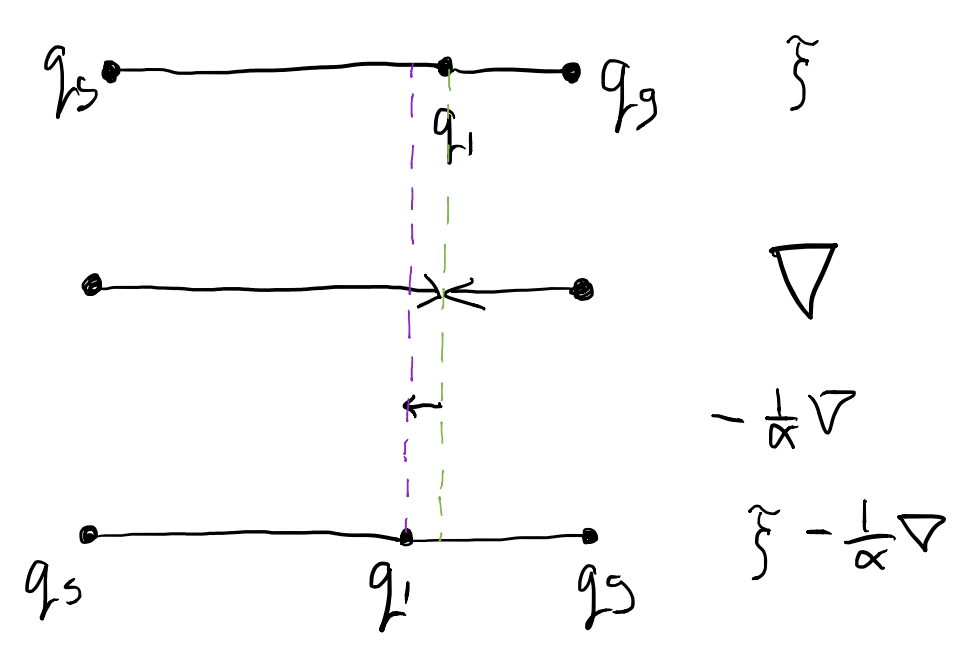
\includegraphics[scale=0.3]{figures/gradient_nudge.png}
\end{center}

\subsection{How to do gradient descent now}
\label{sec:how-do-gradient}

Now that we have our new inner product, how should we do gradient descent? Well, if we modify Equation \eqref{eq:7} to use the $A$-norm instead of the Euclidean norm, we get
\begin{align}
  \label{eq:8}
  \xi_{i+1} &= \text{arg min}_\xi \left\{ \cu[\xi_i] + \nabla_{\xi_i}\cu^\top(\xi - \xi_i) + \frac{1}{2}\alpha \| \xi - \xi_i \|_A^2 \right\}\\
  \intertext{Taking the gradient of the terms inside the curly braces, we get}
            &\phantom{- \text{arg min}_\xi \bigg\{  }0 + \nabla_{\xi_i}\cu + \alpha A (\xi - \xi_i) \label{eq:17} \\
  \intertext{Setting this gradient to zero, we obtain}
  \xi_{i + 1} &= \xi_i - \frac{1}{\alpha} A^{-1}\nabla_{\xi_i}\cu
\end{align}
So here's our equation for gradient descent! But is it correct? Since we're using the new inner product, the term $\nabla_{\xi_i}\cu^\top(\xi - \xi_i)$ should be replaced by $\langle \nabla_{\xi_i}\cu, \xi - \xi_i \rangle_A$, right? Well, that's true, but it's only half of the story: we also have to change from the Euclidean gradient $\nabla_{\xi_i}$ to the $A$-gradient $\nabla^A_{\xi_i}$. We can actually calculate this gradient directly by considering the first-order Taylor expansion of $\cu$ using both inner products:
\begin{align}
  \label{eq:18}
  \cu[\xi] &\approx \cu[\xi_i] + \nabla^A_{\xi_i}\cu^\top A (\xi - \xi_i) \\
\label{eq:19}  &\approx \cu[\xi_i] + \nabla_{\xi_i} \cu^\top (\xi - \xi_i)
\end{align}
These expansions have to be the same, since we're talking about the same function, and the inner products are topologically equivalent, so they have the same notion of limits of small distances. Therefore, the terms on the right must be equal, meaning that
\begin{equation}
  \label{eq:20}
  \nabla_{\xi_i}^A \cu = A^{-1} \nabla_{\xi_i}\cu
\end{equation}
This agrees with our other attempt at an equation for gradient descent! It also makes clear that the new gradient takes the old gradient and `smears it out' along the trajectory. To get a better sense of this, try calculating it for some problems and see what happens!

In summary, it's like we've turned trajectories into elastic bands: it's hard to move one point in the trajectory without moving the other ones along as well.

\section{Student paper presentations}
\label{sec:stud-paper-pres}

Each paper has pro and con presenters. The pro presenter will get approximately 15 minutes to talk, and the con presenter will get approximately 10 minutes to talk.

\subsection{Advice for the pro presenter}
\label{sec:advice-pro-presenter}

Essentially, you should pretend that you wrote the paper, and are presenting it at a conference. Tell the best story you can about the paper.

\begin{itemize}
\item Don't just procedurally go through the paper explaining definitions and theorems in order.
\item Identify the key insight! There will be one main insight in the paper, like ``if the final point of the trajectory can be on a manifold, it's easier to find solutions''. Explain the insight and how it helps.
\item Daniel Dennet: ``You should attempt to re-express your [paper's] position so clearly, vividly, and fairly that [the author would say], `Thanks, I wish I'd thought of putting it that way'.''
\item Use an hourglass structure, where the big ideas come in at the start and the end. First should be the motivation, then the problem statement and why it's hard, then the key insight of the paper, then the nitty-gritty details and results, and at the end restating the key insight and how it helped solve the problem.
\begin{center}
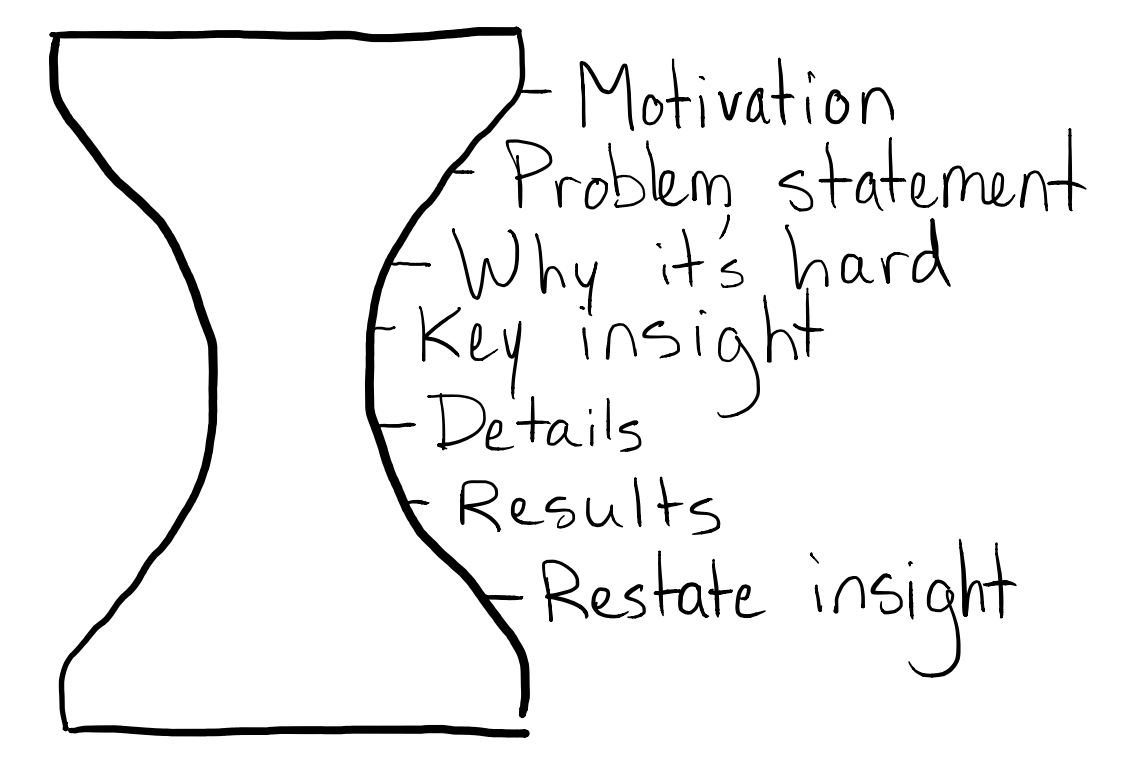
\includegraphics[scale=0.3]{figures/hourglass.png}
\end{center}
\item It would also be good to include demos, videos, etc.
\item Relate back to the lecture material as much as possible. This involves not only translating the notation, but explaining how it fits in with the material we covered, such as showing that something we said was hard was actually easy, or how an algorithm we talked about was developed, or alternatives to an algorithm, etc.
\end{itemize}

\subsection{Advice for the con presenter}
\label{sec:advice-con-presenter}

Essentially, you should talk about how you would improve the paper.

\begin{itemize}
\item Life is easier for you.
\item Be constructive, instead of just saying what's wrong with the paper.
\item One question you could ask is ``What paper would you write?''
\item You can criticise the technical material in the paper, the experiments, or even the key idea, if you can propose improvements.
  \item Relate back to the lecture material as much as possible. This involves not only translating the notation, but explaining how it fits in with the material we covered, such as showing that something we said was hard was actually easy, or how an algorithm we talked about was developed, or alternatives to an algorithm, etc.
\end{itemize}

\subsection{Advice about presenting}
\label{sec:advise-about-pres}

\begin{itemize}
\item It's probably a good idea for many to choose slides instead of a board talk, since board talks are harder to architect, more messy, etc.
\item Board talks are OK too, especially for more theoretical papers. If you do one, you should probably plan what you're going to write ahead of time, be linear (instead of going back and editing things you wrote before), and don't try to invent things on the spot.
\item One common mistake is to put too much text on one slide. Don't do this! Have 1 sentence per slide at most!
\item People can't listen and read at the same time.
\item Have informative titles: not ``Results'', but ``X helped increase Y''
\item Try being visual, using graphs, diagrams and figures. You don't need to copy/paste for paper, and it's better not to do this (see below)
\item Only have 1 point per slide!
\item You can build slides up point by point, starting with a simple graph conveying one point, adding some part that conveys extra, then adding more...
\item Don't put something on a slide if you won't talk about it.
\end{itemize}

\end{document}
%%% Local Variables:
%%% mode: latex
%%% TeX-master: t
%%% End:
